\chapter{General Introduction}
\label{chap:general-introduction}

\section{Motivation and Context}
\label{sec:general-motivation}

Data-driven research increasingly depends on access to detailed datasets, yet the same level of detail that makes data useful can also make it sensitive. In areas such as healthcare, finance, public administration, and social science, individual-level records often cannot be shared freely because of legal, ethical, and institutional constraints. Synthetic data has therefore become an important candidate for privacy-preserving analysis: instead of releasing the original records, a generator produces artificial observations intended to preserve the statistical properties needed for research \cite{rubin1993, little1993, nowok2016}.

The practical value of synthetic data, however, cannot be judged only by whether the generated records look plausible. The central question is whether an analyst using the synthetic data would reach conclusions similar to those obtained from the original data. This is the problem of analytical utility. Prior work distinguishes between broad similarity measures and task-specific utility measures, emphasizing that the right evaluation depends on the downstream analysis being supported \cite{snoke2018}.

This thesis studies synthetic-data utility from that downstream perspective. It asks whether common synthesis methods preserve enough information for two different families of machine-learning and statistical analysis:
\begin{itemize}
  \item \textbf{clustering}, where the relevant utility is structural and geometric;
  \item \textbf{regression}, where the relevant utility is inferential and concerns coefficients, uncertainty, and confidence intervals.
\end{itemize}

\section{Machine-Learning Perspective}
\label{sec:general-ml-perspective}

Machine learning includes a broad set of methods that learn from data rather than relying on explicitly programmed rules. A common taxonomy distinguishes between supervised learning, unsupervised learning, and reinforcement learning. Figure~\ref{fig:ml_taxonomy} summarizes this classification and positions the two analytical settings studied in this thesis.

\begin{figure}[H]
  \centering
  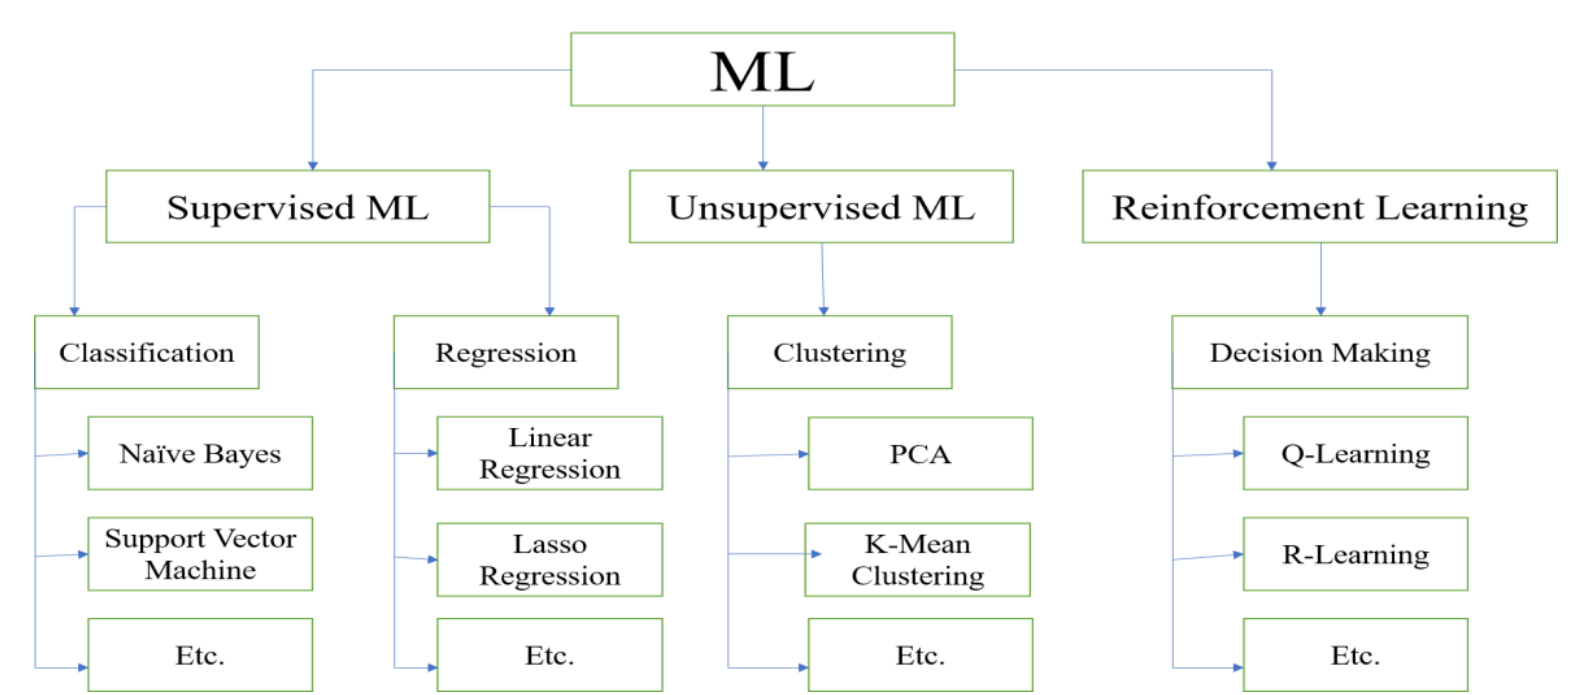
\includegraphics[width=0.85\linewidth]{images/ML_types.png}
  \caption{Taxonomy of common machine-learning paradigms and representative algorithms.}
  \label{fig:ml_taxonomy}
  \source{Compiled by the author}
\end{figure}

Regression belongs to the supervised or model-based inferential setting, because it studies how an outcome changes as a function of predictors. Clustering belongs to unsupervised learning, because it attempts to discover structure without observing ground-truth labels during training. These two settings place different demands on synthetic data. Clustering requires preservation of distances, densities, separability, and cluster geometry. Regression requires preservation of conditional relationships, point estimates, standard errors, and confidence intervals \cite{reiter2003, drechsler2011}.

\section{Problem Statement}
\label{sec:general-problem}

The motivating assumption behind synthetic data is that a generated dataset can act as a useful substitute for the original data. This thesis treats that assumption as empirical rather than automatic. A synthetic generator may preserve marginal distributions while distorting the multivariate structure required by a downstream method. Conversely, a generator may be adequate for one analysis and unsuitable for another.

The synthesis mechanism is especially important. A major part of this thesis evaluates Classification and Regression Trees (CART), as implemented in the \texttt{synthpop} package \cite{nowok2016}. CART is flexible because it models variables through data-driven partitions, but those partitions are axis-aligned. As a result, smooth relationships can become block-like or staircase-shaped after synthesis. The key question is not only whether these artifacts exist, but whether they matter for the analysis that follows.

The thesis is therefore organized around a single claim: synthetic-data utility is not an intrinsic property of a generator alone. It emerges from the interaction between the synthesis method, the data-generating structure, and the downstream analytical task.

\section{Objectives and Research Questions}
\label{sec:general-objectives}

The general objective of this thesis is to evaluate whether synthetic data preserves downstream analytical utility across two complementary settings: clustering and regression.

The specific objectives are:
\begin{enumerate}
  \item To evaluate whether CART-generated synthetic data preserves the geometric structure required by clustering algorithms.
  \item To compare the robustness of centroid-based and connectivity-based clustering under synthetic distortions.
  \item To evaluate whether synthetic data preserves regression coefficients and confidence intervals in linear and logistic models.
  \item To compare CART-based synthesis with parametric synthesis when the downstream analysis has a known model structure.
  \item To identify conditions under which synthetic data remains useful, becomes unstable, or leads to misleading analytical conclusions.
\end{enumerate}

These objectives are addressed through three thesis-level research questions:
\begin{itemize}
  \item \textbf{RQ1:} Does synthetic data preserve the structural geometry required for unsupervised clustering?
  \item \textbf{RQ2:} Does synthetic data preserve the inferential quantities required for regression analysis?
  \item \textbf{RQ3:} How does the match between generator assumptions, data structure, and downstream analytical method determine synthetic-data utility?
\end{itemize}

\section{Structure of the Thesis}
\label{sec:general-structure}

The thesis is divided into two empirical studies under this common framing.

\textbf{Part I} studies structural utility for clustering. It evaluates K-Means and Agglomerative Hierarchical Clustering on CART-generated synthetic datasets, using controlled simulations and structural metrics such as cluster-number recovery, Gini coefficient, Mean Centroid Distance, and Mean Variance Difference.

\textbf{Part II} studies inferential utility for regression. It evaluates linear and logistic regression under CART and parametric synthesis, using Confidence Interval Overlap, Bias Ratio, and Confidence Interval Width Ratio to measure whether synthetic data supports the same statistical conclusions as the original data.

The final discussion integrates both studies and presents the overall thesis conclusion: synthetic data should be selected and validated according to the analysis it is expected to support, not treated as a universally interchangeable replacement for original data.
